\begin{exercise}
For an arbitrary category \(\cat{B}\), consider the domain functor \(\dom : \cat{B}^{\rightarrow} \to \cat{B}\).
\begin{parts}
\part
Describe the fibre category above \(I \in \cat{B}\).
It is usually called the \textbf{opslice category} or simply \textbf{opslice} and written as \(I \setminus \cat{B}\).
\part
Show that \(\dom\) is a fibration (without any assumptions about \(\cat{B}\)).
\part
Show also that for each \(I \in \cat{B}\) the domain functor \(\dom_I : \cat{B} / I \to \cat{B}\) is a fibration.
\end{parts}
\end{exercise}

\begin{partsolution}{i}
For a category \(\cat{B}\) and an object \(I \in \cat{B}\), the category \(I \setminus \cat{B}\) has
\begin{description}
\item[objects]
Morphisms \(\begin{pmatrix}\begin{tikzcd}[row sep=small] I \arrow[d, "\varphi"] \\ X\end{tikzcd}\end{pmatrix}\) in \(\cat{B}\) with domain \(I\).
\item[morphisms]
Given objects \(\begin{pmatrix}\begin{tikzcd}[row sep=small] I \arrow[d, "\varphi"] \\ X\end{tikzcd}\end{pmatrix}\) and \(\begin{pmatrix}\begin{tikzcd}[row sep=small] I \arrow[d, "\psi"] \\ Y\end{tikzcd}\end{pmatrix}\) in \(I \setminus \cat{B}\), a morphism in \(I \setminus \cat{B}\) from the first to the second consists of a morphism \(f : X \to Y\) in \(\cat{B}\) such that the following diagram commutes.
\begin{equation*}
\begin{tikzcd}[column sep=small]
& I \arrow[dl, "\varphi"{above left}] \arrow[dr, "\psi"] \\
X \arrow[rr, "f"] && Y
\end{tikzcd}
\qedhere
\end{equation*}
\end{description}
\end{partsolution}

\begin{partsolution}{ii}
Consider a morphism \(u : I \to J\) in \(\cat{B}\), and another morphism \(\psi: J \to Y\) in \(\cat{B}\) (i.e., an object \(\begin{pmatrix}\begin{tikzcd}[row sep=small] J \arrow[d, "\psi"] \\ Y\end{tikzcd}\end{pmatrix}\) in \(\cat{B}^{\rightarrow}\) over \(J\) with respect to \(\dom : \cat{B}^{\rightarrow} \to \cat{B}\)).
We claim that
\begin{align}
\label{eq:ex:1.1.1.8(ii):lift candidate}
\begin{tikzcd}[ampersand replacement=\&,]
\begin{pmatrix}
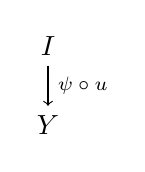
\begin{tikzpicture}
        \node(1){\(I\)}; 
        \node(2)[below of=1]{\(Y\)};
        \draw[->](1)--node[right]{\scriptsize\(\psi \circ u\)} (2);
\end{tikzpicture}
\end{pmatrix}
\arrow[r, "{(\id_Y, u)}"]
\&
\begin{pmatrix}
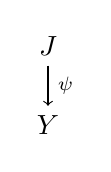
\begin{tikzpicture}
        \node(1){\(J\)}; 
        \node(2)[below of=1]{\(Y\)};
        \draw[->](1)--node[right]{\scriptsize\(\psi\)} (2);
\end{tikzpicture}
\end{pmatrix}
\end{tikzcd}
&& \text{i.e.,}
&&
\begin{tikzcd}[ampersand replacement=\&,]
I \arrow[r, "u"] \arrow[d, "\psi \circ u"{left}] \& J \arrow[d, "\psi"] \\
Y \arrow[r, equal] \& Y
\end{tikzcd}
\end{align}
is a Cartesian lift of \(u\).
Indeed, consider a situation as in the following commutative diagram of solid arrows.
\begin{equation}
\label{eq:ex:1.1.1.8(ii):situation}
\begin{tikzcd}[row sep=small]
\begin{pmatrix}
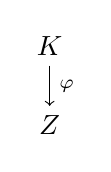
\begin{tikzpicture}
        \node(1){\(K\)}; 
        \node(2)[below of=1]{\(Z\)};
        \draw[->](1)--node[right]{\scriptsize\(\varphi\)} (2);
\end{tikzpicture}
\end{pmatrix}
\arrow[rrd, bend left, near end, "{(g, u \circ v)}"]
\arrow[rd, dashed, "?"] \arrow[dd, -Triangle, "\dom"{left}]
\\[-7ex]
& \begin{pmatrix}
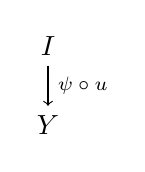
\begin{tikzpicture}
        \node(1){\(I\)}; 
        \node(2)[below of=1]{\(Y\)};
        \draw[->](1)--node[right]{\scriptsize\(\psi \circ u\)} (2);
\end{tikzpicture}
\end{pmatrix}
\arrow[r, "{(\id_Y, u)}"] \arrow[dd, -Triangle, "\dom"]
&
\begin{pmatrix}
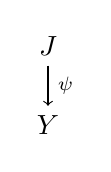
\begin{tikzpicture}
        \node(1){\(J\)}; 
        \node(2)[below of=1]{\(Y\)};
        \draw[->](1)--node[right]{\scriptsize\(\psi\)} (2);
\end{tikzpicture}
\end{pmatrix} \arrow[dd, -Triangle, "\dom"]
\\
K \arrow[rd, "v"]
\\
& I \arrow[r, "u"] & J
\end{tikzcd}
\end{equation}
We must find a unique morphism in \(\cat{B}^{\rightarrow}\) to fill in the dashed ``\(?\)'' arrow in \eqref{eq:ex:1.1.1.8(ii):situation} that makes the diagram commute.
But observe that \eqref{eq:ex:1.1.1.8(ii):situation} is equivalent to the following diagram.
\begin{equation*}
\begin{tikzcd}
K \arrow[r, "v"] \arrow[d, "\varphi"] & I \arrow[r, "u"] \arrow[d, "\psi \circ u"] & J \arrow[d, "\psi"] \\
Z \arrow[r, dashed, "?"] \arrow[rr, bend right, "g"{below}] & Y \arrow[r, equal] & Y
\end{tikzcd}
\end{equation*}
It becomes evident that the unique morphism that fills in the dashed ``\(?\)'' arrow in \eqref{eq:ex:1.1.1.8(ii):situation} to makes the diagram commute is \(? = (g, v)\).
Thus, \eqref{eq:ex:1.1.1.8(ii):lift candidate} is a Cartesian lift of \(u\), and hence \(\dom : \cat{B}^{\rightarrow} \to \cat{B}\) is a fibration.
\end{partsolution}

\begin{partsolution}{iii}
The same proof as in \partref{1}{1}{8}{ii} applies here as well.
Explicitly, fix an object \(I\) in \(\cat{B}\), let \(u : X \to Y\) be a morphism in \(\cat{B}\), and let \(\begin{pmatrix}\begin{tikzcd}[row sep=small] Y \arrow[d, "\psi"] \\ I\end{tikzcd}\end{pmatrix}\) in \(\cat{B} / I\) over \(Y\) relative to the functor \(\dom_I : \cat{B} / I \to \cat{B}\).
Then a straightforward modification of the proof of \partref{1}{1}{8}{ii} shows that
\begin{align*}
\begin{tikzcd}[ampersand replacement=\&,]
\begin{pmatrix}
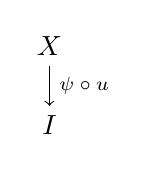
\begin{tikzpicture}
        \node(1){\(X\)}; 
        \node(2)[below of=1]{\(I\)};
        \draw[->](1)--node[right]{\scriptsize\(\psi \circ u\)} (2);
\end{tikzpicture}
\end{pmatrix}
\arrow[r, "u"]
\&
\begin{pmatrix}
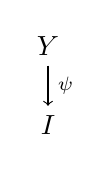
\begin{tikzpicture}
        \node(1){\(Y\)};
        \node(2)[below of=1]{\(I\)};
        \draw[->](1)--node[right]{\scriptsize\(\psi\)} (2);
\end{tikzpicture}
\end{pmatrix}
\end{tikzcd}&& \text{i.e.,}
&&
\begin{tikzcd}[ampersand replacement=\&, column sep=small]
X \arrow[rr, "u"] \arrow[dr, "\psi \circ u"{below left}] \& \& J \arrow[dl, "\psi"] \\
\& I
\end{tikzcd}
\end{align*}
is a Cartesian lift of \(u\), and hence \(\dom_I : \cat{B} / I \to \cat{B}\) is a fibration.
\end{partsolution}